\documentclass[a4]{article}
\usepackage[austrian]{babel}
\renewcommand{\familydefault}{\sfdefault}
\usepackage{amsfonts,latexsym,amssymb,graphicx}
\usepackage[utf8]{inputenc}
%\usepackage[T1]{fontenc}
\title{\bf 183.605 \\ Machine Learning for Visual Computing \\ Aufgabenblock 1}
\author{Michael Reiter}
\date{30. Oktober 2012}
\begin{document}
\noindent

\maketitle

\noindent
Abgabe der Aufgaben 1.1 und 1.2 bis 2.12.2012, 18:00h via TUWEL. \\
\begin{itemize}
\item Lauffähiger MATLAB code in einem zip file (keine Unterverzeichnisse, ein Matlabskript, mit dem alle Ergebnisse erzeugt werden)
\item PDF Dokument mit Experimentergebnissen, Dokumentation und
ausf"uhrlicher Diskussion.
\item Alle Fragen müssen in der Dokumentation beantwortet sein.
\end{itemize}

\section{Aufgabe I}
Ziel dieses Aufgabenblocks ist es, Erfahrung mit dem Aufbau eines einfachen Perzeptrons und Lernverfahren zu sammeln. Aufbauend darauf sollen später Experimente mit einem \emph{Linear Basis Function Model} durchgeführt werden.

\subsection{Teil 1: Einfaches Perzeptron}

\subsubsection{Datengeneration}\label{sec:datageneration}
Schreiben Sie eine Funktion \texttt{[data,target] = genData(n,d)}, die synthetische Daten für ein binäres Klassifikationsproblem generiert. $data$ soll Datenmatrizen, mit $n$ Zeilen (= Anzahl der Beobachtungen) und  $d$ Spalten (=Dimension der Eingabevektoren) enthalten. $target$ enthält einen $n$-Vektor (Zeilenvektor) der zu jeder Beobachtung den entsprechenden Target Wert $\in \left\{-1,1\right\}$ enthält. Sie können obiger Funktion weitere Parameter hinzufügen, mit denen gesteuert werden kann, ob eine linear separierbare oder nicht l.s. Menge generiert werden soll (zB. boolescher Wert).

Generieren sie damit 2 Datens"atze
mit jeweils $100$ $2$-dimensionalen Beobachtungen. Die Eingabedaten sollen mit der Matlab-Funktion $randn$ erzeugt werden, wobei für die 2 Klassen die Eingabevektoren als jeweils $50$ Realisationen einer Normalverteilung ($d$-dimensional) erzeugt werden sollen. Wählen Sie die beiden Mittelwerte und (Ko-) Varianzen für die 2 Klassen so, dass linear separierbarere und nicht linear separierbarere Datens"atze mit jeweils 100 $2$-dimensionalen Beobachtungen mit entsprechenden Target-Werten entstehen. Erzeugen Sie mehrere (mindestens 2) linear separierbare Datensätze mit verschiedenen Mittelwerten und Kovarianzen, sodass der ''Abstand'' der Klassen variiert (minimaler Abstand zweier Beobachtungen aus unterschiedlichen Klassen).

\vspace{2mm}
\noindent {\bf Fragen:}
\begin{itemize}
\item Stellen Sie die Lage der Datenvektoren in $\mathbb{R}^2$ und
ihre labels (Targetwerte) graphisch dar.
\end{itemize}

\subsubsection{Perzeptrontraining}
Schreiben sie eine Funktion, die ein einfaches Perzeptron simuliert,
als Eingabewerte den Gewichtsvektor ${\bf w}$ und Eingabedaten ${\bf x}$
akzeptiert und die Perzeptronausgabe ${\bf y}$ liefert, d.h.
\begin{center}
\texttt{y = perc(w,x)}.
\end{center}
Implementieren Sie sowohl das \emph{online}-Trainingsverfahren als auch das \emph{batch}-Verfahren (siehe Vorlesungsfolien),
d.h. \texttt{w} soll mit einer entsprechenden Matlab Funktion wie folgt ermittelt werden:
\begin{center}
\texttt{w = percTrain(X,t,maxIts,online)}.
\end{center}
Eingabe f"ur den Trainingsalgorithmus sind Trainingsdaten ${\bf X}$,
Targetvektor ${\bf t}$ und eine Obergrenze für die Zahl der
Trainingsiterationen \texttt{maxIts}. \texttt{online} gibt an, ob mittels \emph{online}-Verfahren oder \emph{batch}-Verfahren trainiert wird. Die Rückgabe ist ein weight-Vektor ${\bf w}$.

\vspace{2mm}
\noindent {\bf Fragen:}
\begin{itemize}
\item Untersuchen sie den Trainingsalgorithmus:  Welche Eigenschaften der Daten beeinflussen die durchschnittliche Anzahl an Iterationen bis eine Lösung ${\mathbf w}^*$ gefunden wurde?
\item Welchen Einflu"s hat die Schrittweite?
\item Plotten Sie Daten und Entscheidungsgrenze in $\mathbb{R}^2$
(analog zu Punkt\ref{sec:datageneration}).
\item Wie ist das Verhalten bei nicht linear separierbaren Daten?
\end{itemize}

\subsection{Teil 2: Lineare Regression}

Ziel dieser Aufgabe ist es, Parameteroptimierung auf einer Fehlerfunktion umzusetzen und dabei den Zusammenhang zwischen Modellkomplexität (entspricht in diesem Fall Anzahl der Basisfunktionen) und theoretischem Gesamtfehler zu untersuchen.

\subsubsection{Datengenerierung}
Generieren Sie einen Vektor mit Eingabewerten $x \in [0,5]$ (Zeilenvektor mit 1-dimensionalen Eingabewerten) mit einer Schrittweite von $0.1$ (51 Eingabewerte)
und einen entsprechenden Datenvektor \texttt{y} mit Ausgabewerten $y = 2x^2-Gx+1$, wobei
$G=Gruppennummer$. Diese 51 Punkte sollen zur Visualisierung (Plotten) der gesuchten Funktion herangezogen werden.
Erstellen Sie aus den 51 Punkten eine Trainingsmenge indem Sie jeden 6 Punkt auswählen und
jeweils einen mit $\mathcal{N}(\mu = 0,\sigma = 0.7)$ normalverteilten zufälligen Wert zu $y_i$ addieren um verrauschte Targetwerte $t_i$ zu erzeugen. Die so erzeugte Trainingsmenge enthält $N = 8$ Paare von Beobachtungen $x_i, t_i$. 

\begin{figure}[!h]
\begin{center}
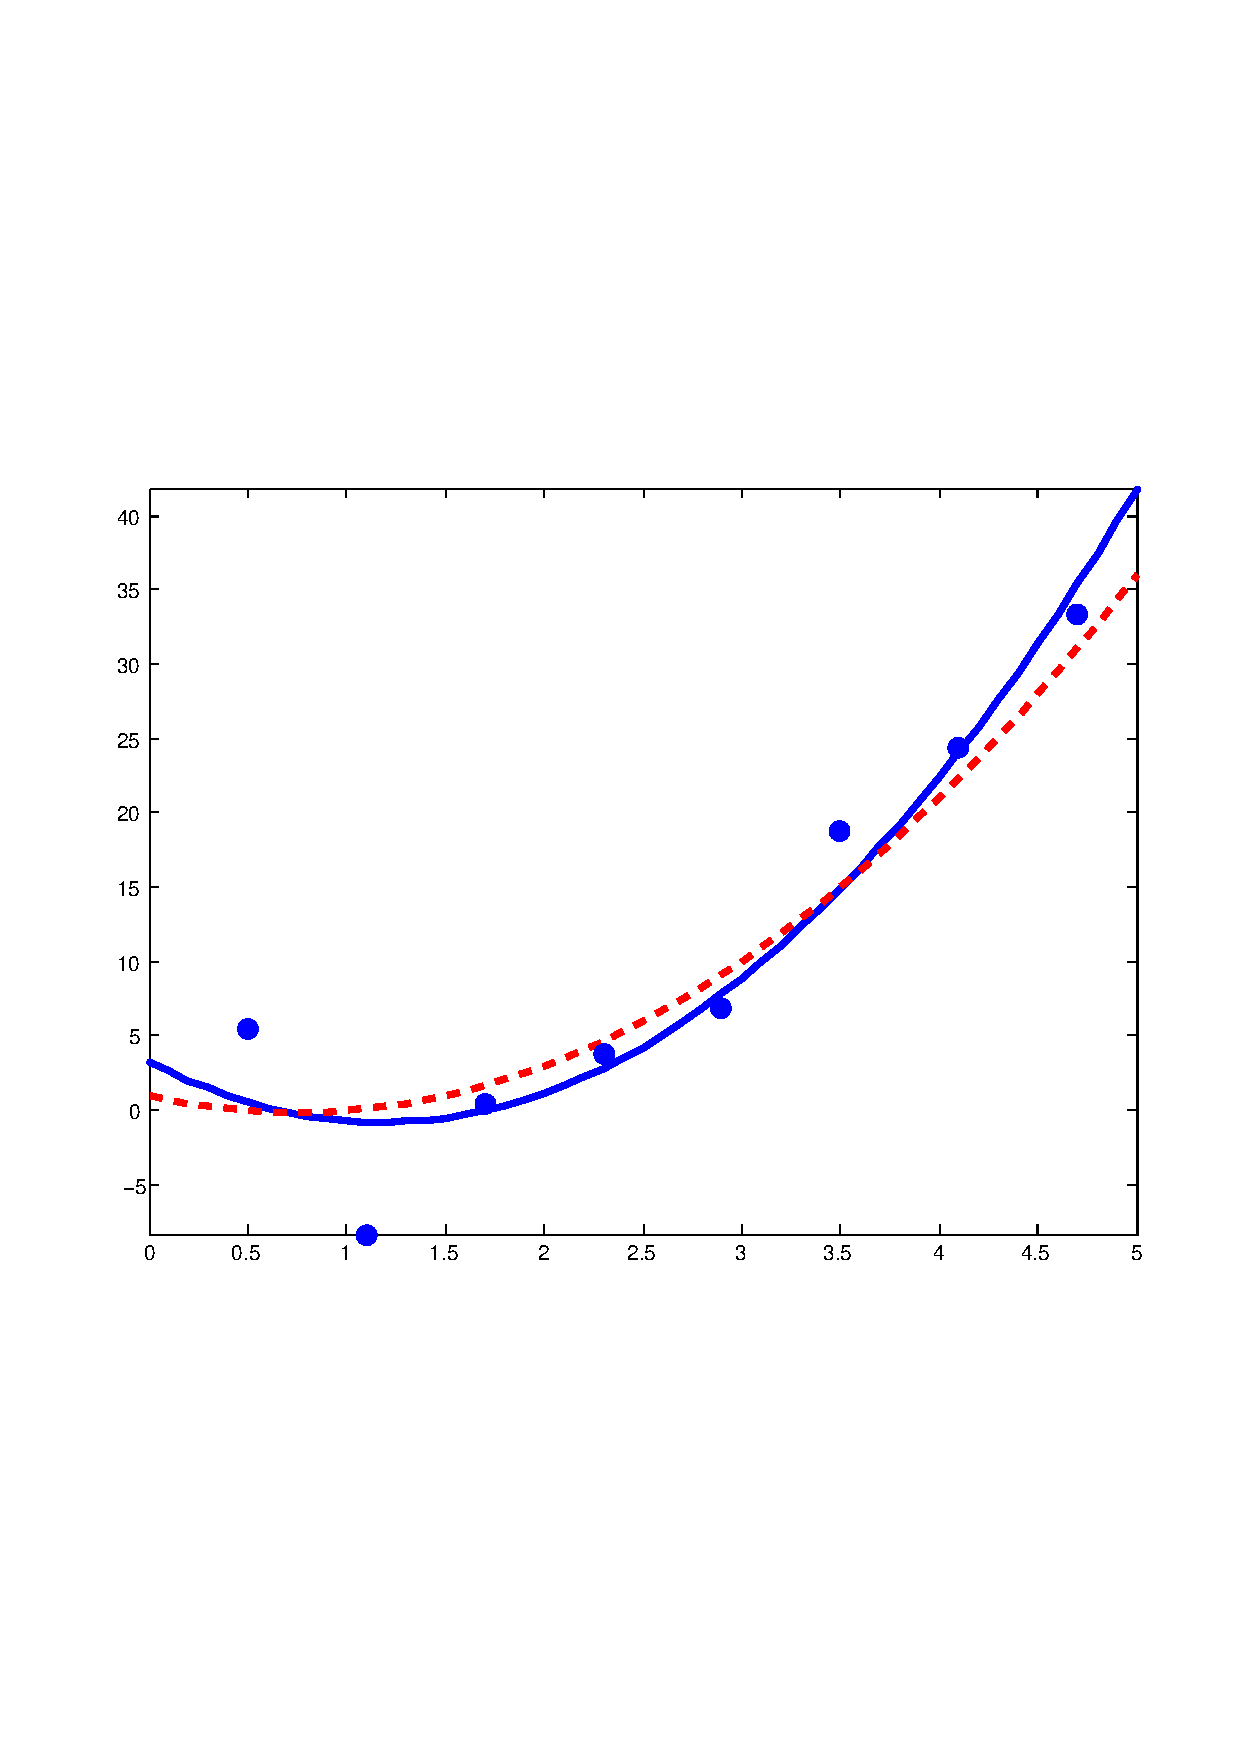
\includegraphics[width=4.5cm]{regression.pdf}
\end{center}
\caption{Beispiel einer wahren Funktion (rot gestrichelte Kurve), der Trainingsmenge mit $N=8$ (blaue Punkte) und dem
dem Ergebnis der Regression (blaue Kurve) mit einem Polynom mit Grad 2.}
\end{figure}

\subsubsection{Basisfunktionen und Parameteroptimierung}

Verwenden Sie eine lineare Einheit (\emph{online} LMS Lernregel) um lineare Regression durchzuf"uhren. Führen Sie die Regression auf transformierten Eingabedaten durch. Verwenden Sie beispielsweise folgende Merkmalstransformation: ${\mathbf \Phi}(x) \rightarrow (1,x,x^2)^T$ (Matlab kann elementweise potenzieren: z.B. \texttt{[x x x].$\wedge$ [0 1 2]}). Hinweis:  Es ist hilfreich w"ahrend des Trainings bereits $y$ und die Vorhersage (Ausgabe der linearen Einheit) zu plotten bzw. die Ver"anderung des Gewichtsvektors zu verfolgen um schnell zu sinnvollen Werten für die Lernrate $\gamma$ zu kommen (m"ogliche Laufzeiteinbu"sen). 

\vspace{2mm}
\noindent {\bf Fragen:}
\begin{itemize}
\item Welchen Gewichtsvektor erhalten Sie mittels Gradientenabstieg auf der quadratischen Fehlerfunktion?
\item Wie können Sie den optimalen Gewichtsvektor ${\mathbf w}^*$ im Fall einer quadratischen Fehlerfunktion in einem Schritt berechnen? Vergleichen Sie das so berechnete Optimum mit dem Ergebnis des Gradientenabstiegs.
\item Untersuchen Sie den Einfluß der Schrittweite $\gamma$ auf das
Konvergenzverhalten. Welches $\gamma$ ergibt eine guten \emph{tradeoff}
zwischen Trainingszeit und Konvergenzverhalten? Gibt es ein $\gamma$,
bei dem ${\mathbf w}$ divergiert?
\end{itemize}

\subsubsection{Modellkomplexität und Modellselektion}
Ergänzen Sie weitere Basisfunktionen ${\mathbf \Phi}(x) \rightarrow (1,x,x^2,x^3,...,x^d)^T$ (und vergrö{\ss}ern Sie ${\mathbf w}$ entsprechend). Berechnen Sie ${\mathbf w}^*$ für mindestens 2000 verschiedene Trainingsmengen mit $\sigma = 0.7$. Schätzen Sie den Erwartungswert und die Kovarianz von ${\mathbf w}^*$ (${\mathbf w^*}$ ist eigentlich ein Schätzer der Koeffizienten der wahren Funktion). 

\vspace{2mm}
\noindent {\bf Fragen:}
\begin{itemize}
\item Wie verhält sich der Erwartungswert und wie die Varianzen aller Koeffizienten in ${\mathbf w}^*$ im Bezug zu $d$? Was können Sie im Speziellen über die Koeffizienten der hinzugefügten Basisfunktionen ($2< j \leq d$) sagen?
\item Plotten Sie für ein fixes $x^*$ (z.B. $x^* = 2$) die mittlere Abweichung der Modellvorhersage von $f_{\mathbf w^*}(x^*)$ vom wahren Funktionswert $f(x^*)$ (anhand der 2000 Trainingsmengen) im Bezug zu $0 \leq j \leq d$ ($d = 0$ bedeutet konstante Funktion).  
\item Welches ${\mathbf w^*}$ erhalten Sie bei einer ungestörten Trainingsmenge im Bezug zu $d$?
\end{itemize}

\end{document}
